\scanpage{11}
\figure{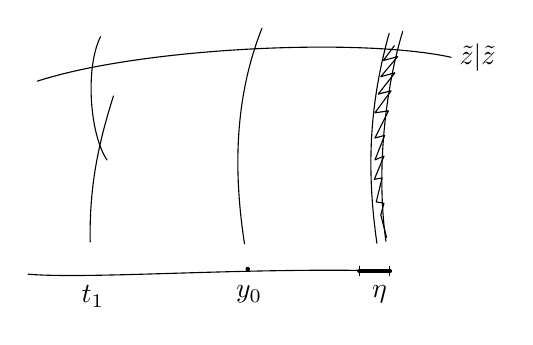
\begin{tikzpicture}[x=.82cm,y=.82cm,line cap=round,line join=round]
\draw (0,0) .. controls (1,-.08) and (3.4,.11) .. (5.60,.05);
\draw[line width=1.7pt] (5.13,.05)--(5.60,.05);
\draw (5.13,-.02)--(5.13,.12) (5.60,-.02)--(5.60,.12);
\fill (3.40,.08) circle (.035);
\node[below] at (1.00,-.03) {$t_1$};
\node[below] at (3.42,-.03) {$y_0$};
\node[below] at (5.44,-.03) {$\eta$};
\draw (.96,.50) .. controls (.94,1.42) and (1.12,2.13) .. (1.32,2.76);
\draw (1.22,1.77) .. controls (.95,2.17) and (.88,3.20) .. (1.12,3.68);
\draw (3.35,.47) .. controls (3.15,1.76) and (3.24,2.85) .. (3.62,3.81);
\draw (5.40,.48) .. controls (5.25,1.54) and (5.26,2.55) .. (5.59,3.73);
\draw (5.54,.51) .. controls (5.37,1.71) and (5.57,3.02) .. (5.80,3.76);
\draw (5.55,.57)--(5.46,.92)--(5.51,1.10)--(5.39,1.12)--(5.48,1.49)--(5.36,1.47)--(5.51,1.83)--(5.37,1.77)--(5.52,2.15)--(5.37,2.11)--(5.58,2.53)--(5.37,2.50)--(5.62,2.84)--(5.42,2.79)--(5.68,3.12)--(5.46,3.06)--(5.72,3.37)--(5.50,3.31)--(5.67,3.54);
\draw (.14,2.99) .. controls (1.74,3.51) and (5.14,3.67) .. (6.55,3.36);
\node[right] at (6.53,3.36) {$\unsure{\tilde z|\tilde{\mathfrak z}}$};
\end{tikzpicture}}

À déterminer a) les noyaux de
\diagram{\begin{tikzcd}[ampersand replacement=\&,row sep=0pt,column sep=2.2em]
\operatorname{Pic}(X^{\unsure{+|'|*}})'\arrow[r] \& \raisebox{-.7ex}{$\deleted{\operatorname{Pic}}J^0(\widetilde X_{\bar\eta})$}\\
\operatorname{Pic}(\widetilde X)'\arrow[r,phantom,"\unsure{\text{---}|\longrightarrow}" description] \& {}
\end{tikzcd}}

b) leur image

\uline{N.B.} $\operatorname{Pic}(\widetilde X_\eta)\longrightarrow\operatorname{Pic}(\widetilde X_{\bar\eta})$ est injectif, donc
le noyau de $\operatorname{Pic}(\widetilde X)^{\deleted{\unsure{'|*}}}\text{---}\operatorname{Pic}(\widetilde X_{\bar\eta})$ \deleted{\illegible{2}}
(égal au noyau de $\operatorname{Pic}(\widetilde X)'\text{---}J^0(\widetilde X_{\bar\eta})$) est
aussi celui de $\operatorname{Pic}(\widetilde X)\text{---}\operatorname{Pic}(\widetilde X_\eta)$, ie
est formé des \uline{classes des diviseurs verticaux}

\deleted{Parmi ceux-ci,} Noter que les div.
verticaux $\widetilde X_y$, pour $y\in\mathbb P^1(k)$, \deleted{($\widetilde X_y$ non \unsure{sing.})}
sont lin. équivalents entre eux, donc à
$\widetilde X_{y_0}=\widetilde Y_0\simeq Y_0$. \deleted{\unsure{Partant|Donc}} Si \inserted{\uline{tous}} les $X_y$ sont \deleted{irr. et}
\deleted{\unsure{div.} \unsure{ver.}} \uline{intègres}, alors le noyau de
$\operatorname{Pic}(\widetilde X)'\longrightarrow\deleted{\operatorname{Pic}}J^0(\widetilde X_{\bar\eta})$ est réduit aux \deleted{classes des} multiples
de \deleted{$\operatorname{cl}(\widetilde X_y)$} la classe \deleted{$\unsure{\widetilde X_y}$} de $\widetilde Y_0$, \deleted{\unsure{Notons} \unsure{pour|que}} \inserted{soit $\tilde\xi_0$}, qui est
% archive sheet number: 10
